\documentclass[10pt]{article}\usepackage[margin=.55in]{geometry}\usepackage[T1]{fontenc}\usepackage{graphicx}\setlength{\parindent}{0pt}\setlength{\parskip}{4pt}\sloppy\begin{document}{\large Native narrow modular power and inverse value bridge}\par The literal value model passed 10 theorem declarations, 7 controls and 17 separate named axiom readbacks. For prime p, canonical nonzero x, and p at most 2\textasciicircum{}32, the native inverse value is canonical and decodes to the field inverse. The power theorem does not require primality.\par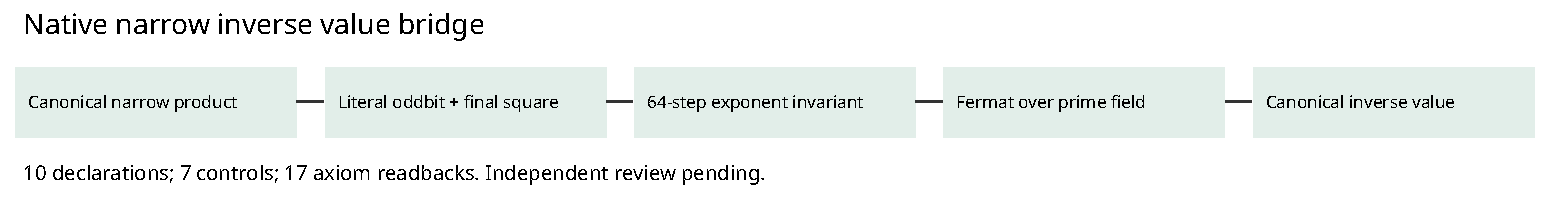
\includegraphics[width=.96\linewidth]{diagram.pdf}\par The transition follows the source order: test the low bit for equality to one, conditionally multiply the accumulator, unconditionally square x, then shift the exponent. This differs from the earlier wide-multiplication model, which skipped the final unused square. The 64-step fuel covers every UInt64 exponent; the inductive premise is exponent less than 2\textasciicircum{}fuel. Canonical operands and the modulus bound ensure each narrow product is below 2\textasciicircum{}64.

Controls cover exponent zero, modulus two, odd and even exponents, the final square, the maximum UInt64 exponent, and a multiplication counterexample outside the modulus bound. At p=4294967297 and x=4294967296, native wrapped x*x mod p is zero while the natural product mod p is one. The deliberately wrong inverse 3 inverse modulo7 equals4 was rejected.

Two bounded software attempts used 42.937794 seconds in total. Attempt1 stopped at an unresolved imported helper name; its exact source and failure are retained. Attempt2 passed and checked 28,785 dependency/toolchain file hashes unchanged. The frozen ceiling was three attempts of at most120 seconds each,360 seconds cumulative, one Lean worker,8GiB address space,3500MiB Lean heap and explicit stack limits. No third attempt ran.

Prior work: fast-call-and-word-reviews/batch-review/input/Wide.lean.txt and Inversion.lean.txt, their independent REVIEW.md, and WordComparator.mul\_decode. Fermat and canonical decoding are reused. Exact native source is recover\_boundary\_impl.rs, bound in result.json and source-fidelity.csv. No novelty claim is made.

Scope: the theorem supplies the value-level inverse premise used by the reviewed normalization component. Ops.i counter effects and overflow are excluded. Native pivot search, swap, zero-prefix propagation, concrete array loop composition and full solve4 return remain separate source bridges. Shared dependency binary hashes are bound; an independent binary/kernel rechecker was not run. Independent source-fidelity review is pending publication.

The archive preserves both attempts, exact imported local source/binary closure and recursive dependency/toolchain inventories. The first failure did not reach its planned post-hash check; the final passing attempt did. The axiom allowlist is propext, Classical.choice and Quot.sound. No scientific trajectories or timing comparison were executed.
\end{document}